% Archivo generado automáticamente con los problemas
\section*{Problems}
Sección: 24_Implications_of_unitarity
Páginas: 496-497
Contenido:
24.1 In this problem you will show how the cutting rules can be obtained directly from
contour integration.
(a) Where are the poles in the integrand in Eq. (24.29) in the complex k0 plane?
(b) Close the contour upward and write the result as the sum of two residues. Show
that one of these residues cannot contribute to the imaginary part of M.
(c) Evaluate the imaginary part of the amplitude by using the other pole. Show that
you reproduce Eq. (24.33).
(d) Now consider a more complicated 2 →3 process:
p1
p2
p4
p3
p5
Explore the pole structure of this amplitude in the complex plane and show that
the imaginary part of this amplitude is given by the cutting rules.

24.2 Derive the spectral representation for a Dirac spinor.

24.3 Derive the partial wave unitarity bound for elastic scattering for a theory with
scalars only.

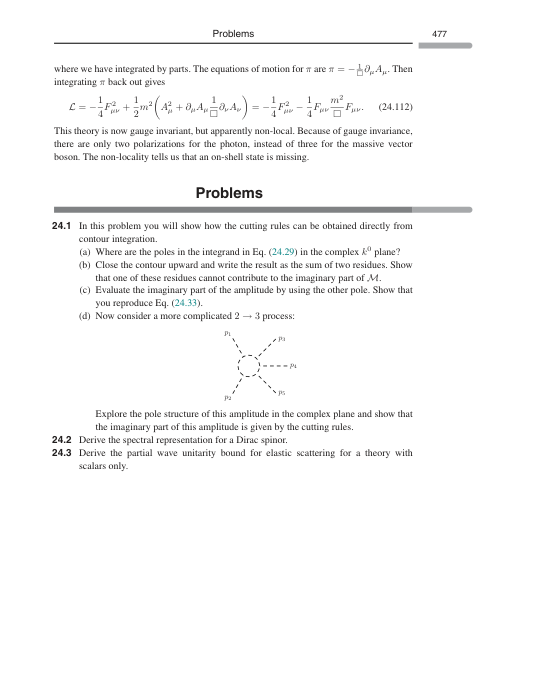
\includegraphics{./figs/24_Implications_of_unitarity_page_497.png}

---

